\documentclass[10pt,openany,a4paper]{article}
\usepackage{graphicx} 
\usepackage{multirow}
\usepackage{enumitem}
\usepackage{amssymb}
\usepackage{amsmath}
\usepackage{xcolor}
\usepackage{color, colortbl}
\usepackage{soul}
\usepackage{cancel}
\usepackage{geometry}
	\geometry{
		total = {160mm, 237mm},
		left = 25mm,
		right = 35mm,
		top = 30mm,
		bottom = 30mm,
	}
\usepackage{fancyhdr}
\usepackage{tikz, pgfplots, tkz-euclide,calc}
    \usetikzlibrary{patterns,snakes,shapes.arrows}

\newcommand{\R}{\mathbb{R}}
\newcommand{\N}{\mathbb{N}}
\newcommand{\jawab}{\textbf{Jawab}:}
\renewcommand{\headrulewidth}{0pt}
\pagestyle{fancy}

\begin{document}
\fancyfoot[C]{\raisebox{.5ex}{\rule{0.5cm}{.4pt}}o0o\raisebox{.5ex}{\rule{0.5cm}{.4pt}}}

\begin{tabular}{r c l}
    \includegraphics[width=2cm]{ITS.png}
     &\begin{tabular}{lcll}
        \multicolumn{4}{c}{\begin{tabular}{c}
          \MakeUppercase{evaluasi tengah semester genap 2022/2023}\\
          \MakeUppercase{departemen matematika fsad its}\\
          \MakeUppercase{program sarjana}\\
     \end{tabular}}\\
     \\
          Matakuliah&:&\multicolumn{2}{l}{Analisis 2}\\
          Hari, Tanggal&:&\multicolumn{2}{l}{Rabu, 29 Maret 2023}\\
          Waktu / Sifat&:&\multicolumn{2}{l}{11:00-12:10 (100 menit) / \textit{Closed Book}}\\
          Kelas, Dosen&:&A.&Dr. Mahmud Yunus, M.Si.\\
          &&B&Dr. Rinurwati, M.Si. \& Sunarsini, S.Si, M.Si.\\
          &&C&Drs. Sadjidon, M.Si.
     \end{tabular}
     & 
     \includegraphics[width=2cm]{M.png}
     \\ \hline
\multicolumn{3}{|l|}{\MakeUppercase{harap diperhatikan !!!}}\\
\multicolumn{3}{|l|}{Segala jenis pelanggaran (mencontek, kerjasama, dsb) yang dilakukan pada saat ETS/EAS}\\
\multicolumn{3}{|l|}{akan dikenakan sanksi pembatalan matakuliah pada semester yang sedang berjalan.}\\
\hline
\end{tabular}

\begin{enumerate}
    \item Diketahui $f:[a,b]\to\R$ suatu fungsi \textit{monotone} pada $[a,b]$. Apakah $f$ terintegral
    pada $[a,b]$? Jika "ya", buktikan; jika "tidak", berikan satu contoh penyangkalnya.\\
    \jawab\\
    \st{Jelas Hal ini sesuai teorema di buku}:v\\
    Asumsikan $f$ naik pada $I=[a,b]$ (boleh juga diasumsikan $f$ turun). Partisi interval menjadi
    $n$ subinterval yang panjangnya yaitu $I_k=[x_{k-1},x_k]$ dengan $||I_k||=x_k-x_{k-1}=\dfrac{b-a}{n}$ untuk $k=1,2,...,n$. 
    Lalu kontruksikan sebuah partisi $\mathcal{P}_n$ yang dimana
    \[\mathcal{P}_n:=\left\{I_1,I_2,...,I_n\right\}\]
    Ilustrasikan agar mempermudah bayangan kita
    \begin{center}
        \begin{tikzpicture}[xscale=1.5,yscale=0.8]
            \draw[-Latex] (0,0) -- (4.2,0) node[right] {$x$};
            \draw[-Latex] (0,0) -- (0,5) node[above] {$f(x)$};
            
            \draw[shift={(0.5,0)},color=black] node[below left] {\small{$x_0=a$}};
            \draw[shift={(1,0)},color=blue] node[below] {\small{$x_1$}};
            \draw[shift={(1.5,0)},color=blue] node[below] {\small{$x_2$}};
            \draw[shift={(2,0)},color=blue] node[below] {\small{$\dots$}};
            \draw[shift={(2,1)},color=blue] node[below] {\small{$\dots$}};
            \draw[shift={(2.5,0)},color=blue] node[below] {\small{$x_{n-1}$}};
            \draw[shift={(3,0)},color=black] node[below right] {\small{$x_n=b$}};
                        
            \draw[thick,domain=0.5:3,smooth] plot (\x,{(1.6)^\x}) node [right] {$f$};

            \draw[thin,dashed,smooth] (0.5,0)--++(0,{(1.6)^(0.5)});
            \draw[thin,dashed,smooth,blue] (1,0)--++(0,{(1.6)^(1)});
            \draw[thin,dashed,smooth,blue] (1.5,0)--++(0,{(1.6)^(1.5)});
            \draw[thin,dashed,smooth,blue] (2.5,0)--++(0,{(1.6)^(2.5)});
            \draw[thin,dashed,smooth] (3,0)--++(0,{(1.6)^(3)});
        \end{tikzpicture}
    \end{center}
    Karena $f$ monoton, maka $f(x_k)\leq f(x_{k+1})$ untuk $x_k<x_{k+1}$. Sehingga bisa 
    didefinisikan komponen darbouxnya sebagai berikut
    \begin{flalign*}
        m_k&=\inf\{f(x)\,|\,x\in I_k\}=f(x_{k-1})\\
        M_k&=\sup\{f(x)\,|\,x\in I_k\}=f(x_{k})
    \end{flalign*}
    Kemudian didapatkan jumlahan atas dan jumlahan bawah
    \begin{flalign*}
        L(f;\mathcal{P}_n)&=\sum_{k=1}^{n}m_k(x_k-x_{k-1})=\sum_{k=1}^{n}f(x_{k-1})\dfrac{b-a}{n}\\
        U(f;\mathcal{P}_n)&=\sum_{k=1}^{n}M_k(x_k-x_{k-1})=\sum_{k=1}^{n}f(x_{k})\dfrac{b-a}{n}\\
    \end{flalign*}
    \newpage
    \begin{figure}
        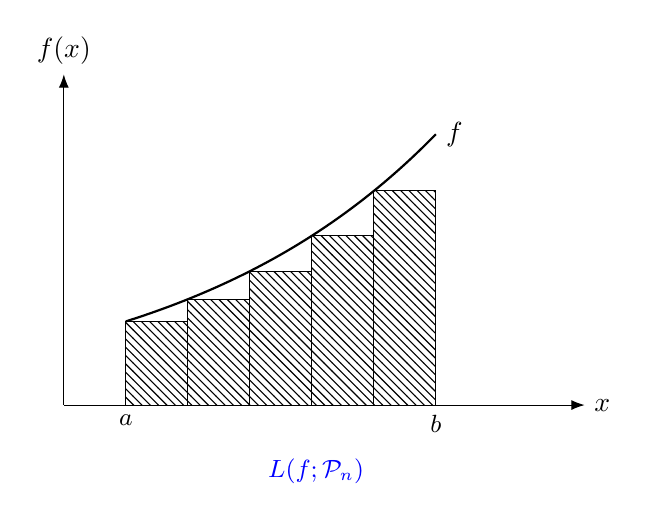
\begin{tikzpicture}[xscale=1.5,yscale=0.8,scale=1.05,left]
            \draw[-Latex] (0,0) -- (4.2,0) node[right] {$x$};
            \draw[-Latex] (0,0) -- (0,5) node[above] {$f(x)$};
            
            \draw[shift={(2.5,-1)},color=blue] node[] {\small{$L(f;\mathcal{P}_n)$}};
            \draw[shift={(0.5,0)},color=black] node[below] {\small{$a$}};
            \draw[shift={(3,0)},color=black] node[below] {\small{$b$}};
                        
            \draw[thick,domain=0.5:3,smooth] plot (\x,{(1.6)^\x}) node [right] {$f$};

            \draw[fill=lightgray,pattern=north west lines,thin](0.5,0)rectangle(1,{(1.6)^(0.5)});
            \draw[fill=lightgray,pattern=north west lines,thin](1,0)rectangle(1.5,{(1.6)^(1)});
            \draw[fill=lightgray,pattern=north west lines,thin](1.5,0)rectangle(2,{(1.6)^(1.5)});
            \draw[fill=lightgray,pattern=north west lines,thin](2,0)rectangle(2.5,{(1.6)^(2)});
            \draw[fill=lightgray,pattern=north west lines,thin](2.5,0)rectangle(3,{(1.6)^(2.5)});
        \end{tikzpicture}
        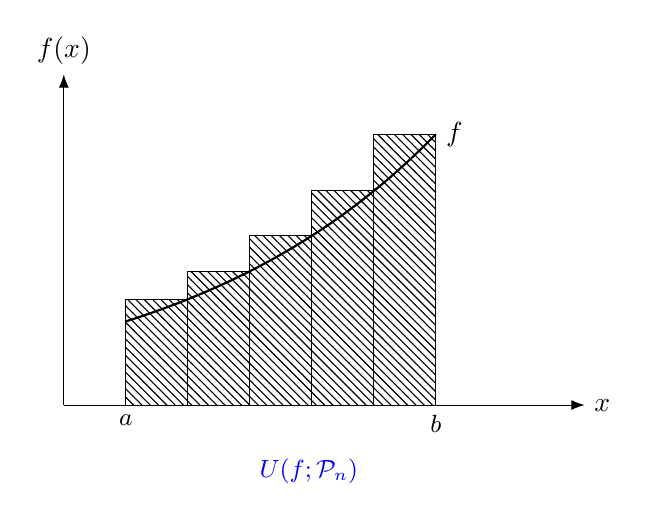
\begin{tikzpicture}[xscale=1.5,yscale=0.8,scale=1.05,right]
            \draw[-Latex] (0,0) -- (4.2,0) node[right] {$x$};
            \draw[-Latex] (0,0) -- (0,5) node[above] {$f(x)$};
            
            \draw[shift={(1.5,-1)},color=blue] node[] {\small{$U(f;\mathcal{P}_n)$}};
            \draw[shift={(0.5,0)},color=black] node[below] {\small{$a$}};
            \draw[shift={(3,0)},color=black] node[below] {\small{$b$}};
                        
            \draw[thick,domain=0.5:3,smooth] plot (\x,{(1.6)^\x}) node [right] {$f$};

            \draw[fill=lightgray,pattern=north west lines,thin](0.5,0)rectangle(1,{(1.6)^(1)});
            \draw[fill=lightgray,pattern=north west lines,thin](1,0)rectangle(1.5,{(1.6)^(1.5)});
            \draw[fill=lightgray,pattern=north west lines,thin](1.5,0)rectangle(2,{(1.6)^(2)});
            \draw[fill=lightgray,pattern=north west lines,thin](2,0)rectangle(2.5,{(1.6)^(2.5)});
            \draw[fill=lightgray,pattern=north west lines,thin](2.5,0)rectangle(3,{(1.6)^(3)});
        \end{tikzpicture}
    \end{figure}
    Kurangkan kedua persamaan diatas sehingga menjadi
    \begin{flalign*}
        U(f;\mathcal{P}_n)-L(f;\mathcal{P}_n)&=\sum_{k=1}^{n}f(x_{k})\dfrac{b-a}{n}-\sum_{k=1}^{n}f(x_{k-1})\dfrac{b-a}{n}\\
        &=\dfrac{b-a}{n}\sum_{k=1}^{n}(f(x_{k})-f(x_{k-1}))\\
        &=\dfrac{b-a}{n}\left((\cancel{f(x_{1})}-f(x_{0}))+(\cancel{f(x_{2})}-\cancel{f(x_{1})})+\cancel{...}+(f(x_{n})-\cancel{f(x_{n-1})})\right)\\
        &=\dfrac{b-a}{n}(f(x_{n})-f(x_{0}))\\
        &=\dfrac{b-a}{n}(f(b)-f(a))
    \end{flalign*}
    Sekarang untuk setiap $\varepsilon>0$, pilih $n$ dimana $n>\dfrac{(b-a)(f(b)-f(a))}{\varepsilon}$. sehingga didapatkan
    \[U(f;\mathcal{P}_n)-L(f;\mathcal{P}_n)<\varepsilon\]
    $\therefore$ Dengan kriteria keintegralan dapat disimpulkan bahwa $f$ terintegral Darboux pada $[a,b]$.

    \item Diberikan barisan fungsi $(f_n)$ yang didefinisikan dengan $f_n(x):=\dfrac{x^n}{1+x^n}$ untuk 
    $x\in[1,2]$ dan $n\in\N$. Selidiki konvergensi barisan fungsi $(f_n)$ tersebut pada $[1,2]$, 
    apakah konvergen titik-demi-titik ataukah seragam.\\
    \jawab\\
    LEMMA. \textit{Barisan $(f_n(x))$ di $A\subseteq\R$ dikatakan konvergen ke $f(x)$ pada $A$ jika dan hanya jika untuk setiap $\varepsilon>0$ dan $x\in A$ terdapat $N(\varepsilon,x)\in\N$ sedemikian sehingga jika $n\geq N(\varepsilon,x)$, maka}.
    \[|f_n(x)-f(x)|<\varepsilon\]
    Perbedaan konvergen titik demi titik dan seragam
    \begin{center}
        \begin{tabular}{|c|c|c|c|}
            \hline
            \rowcolor{lightgray}
            $N(...)$&$N$&$N(\varepsilon)$&$N(\varepsilon,x)$\\
            \hline
            Konvergen T-D-T&\checkmark&\checkmark&\checkmark\\
            Konvergen seragam&\checkmark&\checkmark&$\times$\\
            \hline
        \end{tabular}
    \end{center}
    AKIBAT. \textit{Barisan $(f_n)$ terbatas pada $A\subseteq\R$ konvergen seragam di $A$, maka $(f_n)$ juga konvergen titik-demi-titik pada $A_0$}.\\

    Sehingga kita sebaiknya mengecek apakah $(f_n)$ konvergen seragam di $[1,2]$.\\

    LEMMA. \textit{Barisan $(f_n(x))$ di $A\subseteq\R$ dikatakan konvergen seragam ke $f(x)$ pada $A$ jika dan hanya jika $\sup_{x\in A}\left|f_n(x)-f(x)\right|=0$}.\\

    Karena $f_n(1)=\dfrac{1^n}{1+1^n}=\dfrac{1}{2}$, maka dapat diasumsikan barisan $(f_n)$ 
    akan konvergen ke $f(x)=\dfrac{1}{2}$ untuk setiap $x\in[1,2]$. Sehingga diperoleh
    \[\sup_{x\in [1,2]}\left|\dfrac{x^n}{1+x^n}-f(x)\right|=\left|\dfrac{2^n}{1+2^n}-\dfrac{1}{2}\right|\to\left|1-\dfrac{1}{2}\right|=\dfrac{1}{2}\]
    Karena tidak menuju $0$, maka $(f_n)$ tidak konvergen seragam.\\

    Selanjutnya untuk konvergen TDT, step-step pembuktiannya sebagai berikut:
    \begin{enumerate}[label=(\arabic*)]
        \item Pada soal sudah diketahui $f_n(x)=\dfrac{x^n}{1+x^n}=1-\dfrac{1}{1+x^n}$ untuk 
        $x\in[1,2]$, Lalu Asumsikan
        \[f(x)=\begin{cases}
            \frac{1}{2},\quad&x=1\\
            1,\quad&x\in(1,2]
        \end{cases}\]
        (Untuk $f(x)$ bisa dicari dibelakang layar).
        \item Untuk $x=1$ jelas konvergen, sekarang tinjau untuk $x\in(1,2]$.
        \begin{flalign*}
            \left|f_n(x)-f(x)\right|&=\left|1-\dfrac{1}{1+x^n}-1\right|\\
            &=\left|\dfrac{1}{1+x^n}\right|\\
            &\leq\left|\dfrac{1}{x^n}\right|\\
            &\leq\left|\dfrac{1}{n}\right|
        \end{flalign*}
        \item Pilih $N(\varepsilon)=\dfrac{1}{\varepsilon}$, sehingga untuk $n\geq N(\varepsilon)$ berlaku
        \[\left|f_n(x)-f(x)\right|\leq\dfrac{1}{n}<\varepsilon\]
    \end{enumerate}
    $\therefore\,(f_n)$ di $[1,2]$ konvergen titik demi titik, namun tidak dengan konvergen seragam.

    \item Diberikan barisan fungsi $(f_n)$ dengan $f_n(x):=\dfrac{nx}{1+nx}$ untuk $x\in[0,1]$ dan $n\in\N$.
    Tunjukkan bahwa barisan $(f_n)$ tersebut konvergen ke suatu fungsi yang terintegral pada $[0,1]$ dan
    \[\lim_{n\to\infty}\int_{0}^{1}f_n(x)\,dx=\int_{0}^{1}\lim_{n\to\infty}f_n(x)\,dx\]
    \jawab\\
    TEOREMA. \textit{Misalkan $(f_n)$ suatu barisan fungsi di $\mathcal{R}[a,b]$ yang konvergen pada $[a,b]$ ke suatu fungsi $f\in \mathcal{R}[a,b]$. Jika Terdapat $B>0$ sehingga $|f_n(x)|\leq B$ untuk semua $x\in[a,b]$ dan $n\in\N$, maka berlaku}.
    \[\int_{a}^{b}f=\lim_{n\to\infty}\int_{a}^{b}f_n\]

    Untuk menggunakan teorema diatas, kita perlu membuktikan bahwa $f_n(x)=\dfrac{nx}{1+nx}=1-\dfrac{1}{1+nx}$
    terintegral di $[0,1]$. Dapat dicek dengan mudah bahwa $f_n(x)$ monoton naik untuk setiap $n\in\N$ dan 
    $x\in[0,1]$, sehingga menurut salah satu teroema mengatakan jika $f_n(x)$ monoton maka 
    $f_n(x)$ terintegral di $[0,1]$.\\

    Selanjutnya diketahui bahwa $f_n(x)$ konvergen ke $f(x)=\begin{cases}
        0,\quad&x=0\\
        1,\quad&0<x\leq 1
    \end{cases}$ yang dimana jelas bahwa $f\in\mathcal{R}[0,1]$ seperti yang sudah diketahui 
    sebelumnya.\\

    Karena $f_n(x)$ konvergen, maka $f_n(x)$ juga terbatas lebih tepatnya di $f(x)=1$ yang dapat
    ditulis $|f_n(x)|\leq 1$ untuk semua $x\in[0,1]$ dan $n\in\N$. Hal tersebut mengindikasikan bahwa terdapat $B=1$ dimana 
    $|f_n(x)|\leq B$ untuk setiap $x\in[0,1]$ dan $n\in\N$ yang mengimplikasikan bahwa
    \[\int_{0}^{1}f=\lim_{n\to\infty}\int_{0}^{1}f_n\]

    Karena $(f_n)$ konvergen ke $f$, maka dapat ditulis $\lim_{n\to\infty}f_n=f$. Oleh karena itu,
    persamaan sebelumnya bida diubah menjadi
    \[\int_{0}^{1}\lim_{n\to\infty}f_n=\lim_{n\to\infty}\int_{0}^{1}f_n\]

    \item Tunjukkan bahwa $\lim((\sin{\pi x})^{2n})$ ada untuk semua $x\in\R$, dan dapatkan 
    nilai limit tersebut.
    \jawab\\
    "nilai limit" yang dimaksud di soal adalah sebuah fungsi, sebab barisan diatas merupakan
    barisan fungsi. Oleh karena itu perlu kita cari konvergen kemana barisan fungsi $(\sin{\pi x})^{2n}$.\\
    Misalkan $I:=\left\{\left.\dfrac{1}{2},\dfrac{3}{2},\dfrac{5}{2},...,\dfrac{2k-1}{2}\right|k\in\N\right\}$, 
    Sehingga untuk $x\in I$ didapatkan
    \[\lim((\sin{\pi x})^{2n})=\lim((\pm 1)^{2n})=\lim(1^n)=1\]
    Sedangkan untuk $x\in\R\setminus I$ didapatkan fakta bahwa $0\leq\sin^2{\pi x}<1$, 
    Akibatnya
    \[\lim((\sin{\pi x})^{2n})=0\]
    Dari dua hasil perhitungan diatas, didapatkan bahwa barisan fungsi tersebut konvergen ke 
    suatu fungsi $f(x)$ yaitu
    \[f(x)=\begin{cases}
        0,\quad& x\in\R\setminus I\\
        1,\quad& x\in I
    \end{cases}\]
\end{enumerate}
\end{document}
